\documentclass{diary}

\title{生活日记 \\{\small Plain Life and Wonderful Moments}}
\author{Emrys}

%指定起止日期
\BeginAt[2025]{06}{09}   % 起始日期
\EndAt[\getYear]{\getMonth}{\getDay} % 最后一次编译当天的日期 可不修改

%指定主字体
\setCJKmainfont{华文行楷}  
\setmainfont{Times New Roman}

\begin{document}
\maketitle

\Address[江苏][南京]
\Date{2025}{6}{9}[\sun]%
今天是2025高考的最后一天

回想去年这时候,不免有些感慨

匆匆的,一年时光已流逝

似乎发生了很多很多事

在人生的十字路口

我也做了很多很多个选择

但我感觉我的高考,我的高中生活

一切都还历历在目,是那么熟悉而久违

高中总是充满着紧张与忐忑

尽管我表面上总是风平浪静

或许是我早已习惯一个人闭环

我不会后悔高中的种种选择

也不会怀疑这一年所走的路

一切都是我该走的,该经历的

所有的来时路

铺就来独一无二的我

也照亮了前方我该走的路


\Date{2025}{6}{19}[\winkSmile]%
今天考大雾期末,
老师也太好了看我写错了,
还给我指出来让我检查,
不仅如此,
后面绕了一圈回来,
我改完了在检查下一面,
他先看了看我后一面,点了点头
再做了几遍让我翻面的手势,
一开始我还没看明白hhh,
翻面之后,
看我改了过来才离开,
虽然其实一开始我本来就在检查那题,
觉得我自己写错了。\par
太倒霉了,
复习数分任重而道远,
想题目想着想着,
给泡面倒了一碗冷水,
尽管我倒了大部分水出去再加热水,
还是没泡开,
不过后面我发现
那个泡面里的卤蛋的包装竟然是开的,
不免怀疑泡面是不是也有问题,
还好没吃hhh,
也算是因祸得福。

\Date{2025}{6}{20}[\confused]%
本来觉得数分考的蛮好的,
现在看来又是一坨大便,
唉,
感觉分数要很不如意了,
上学期差不多也这样总评就75,
感觉别人都八九十,
今晚好好复习高代吧,争取考好点,
暑假不能摆烂啊
好好学习,提升自己,
不要沉迷低级趣味,对现阶段无用的事,
不过有一说一,
物理考的蛮好,
一学期没学,期末速通几天,
就99hhh,
上学期解析几何也是,
速通几天喜提99。

\Date{2025}{7}{2}[\nerdSmile]%
今天第一次进厨房,中午尝试着做番茄炒蛋,结果番茄是番茄,蛋是蛋的,卖相更是一言难尽,干巴巴的,明明都倒了很多水。\par
晚上我决定退一步,先学着做面和煎蛋,虽然蛋焦了点,但都凑活着能吃,鼓励自己再接再厉。\\

\begin{center}
    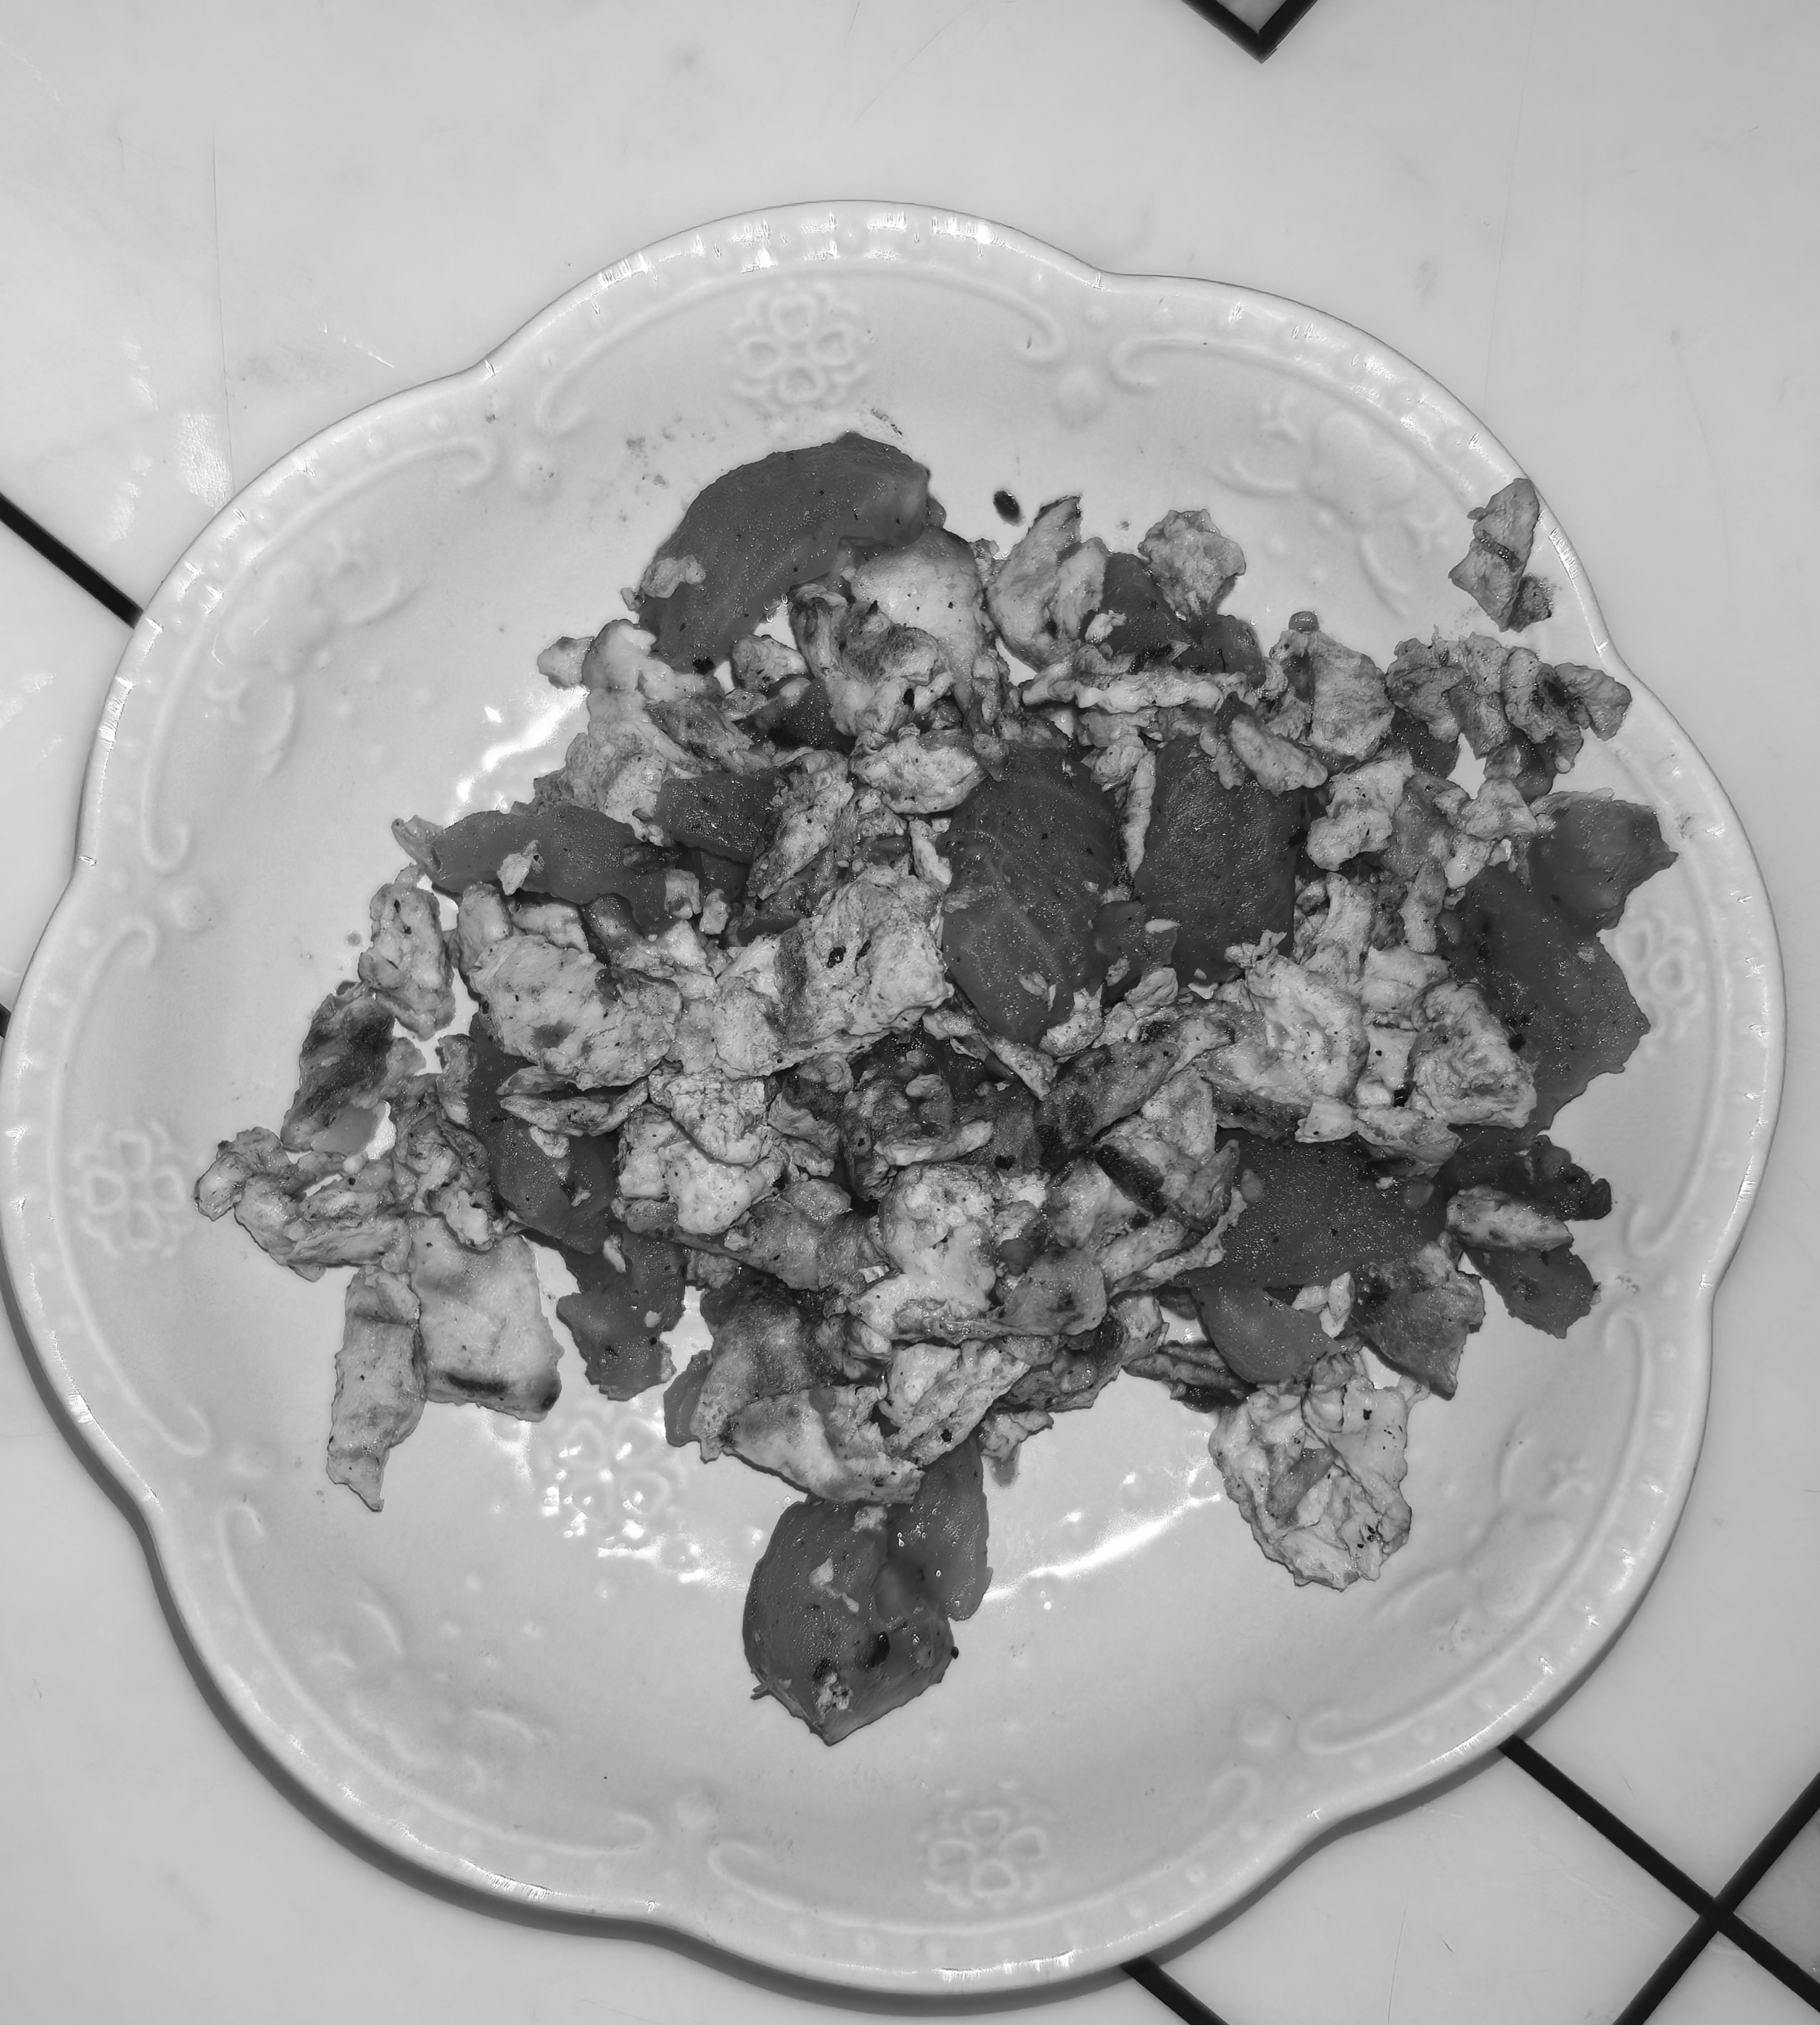
\includegraphics[width=0.5\linewidth,height=0.3\paperheight]{20250702.jpg}
\end{center}

\Date{2025}{7}{3}[\rainy]%
窗外突然下起大雨,不由得内心觉得很安逸,我在房间里学习,一切似乎都是那么的美好惬意。最近天气一直很热,下场大雨感觉凉快了不少,也有可能只是我在空调房里哈哈哈。从小我似乎就对雨天有种特殊的情感,仿佛下雨天我和这个世界的距离拉近了,我更加真切地聆听这个世界的心跳,似乎,天地间只有我一人,听雨的声音,我的思绪也跟着滴滴答答。

\Date{2025}{7}{8}[\simpleSmile]%
这个世界上的善良的人还是很多的,今天骑着电动车在路上,忽然有个阿姨骑着摩托车从我旁边经过,我可以确定我和她素未谋面,可以说是毫无瓜葛,但她出乎我意料地,在骑过我身边的时候,提醒我前面有交警要带头盔,一开始我没有听清,不明所以,她骑到前面一段回头看了我一眼没反应,又大声喊了一遍,前面有交警,忽然一丝温暖淌进心间,人与人之间或许有时候并不一定要靠什么连接,这也许就是人性的可贵。

\Date{2025}{7}{17}[\hot]%
\vspace{-1.5em}
\setlength{\columnsep}{2em}
\begin{wrapfigure}{l}{0.3\linewidth} 
  \vspace{-0.8em}
  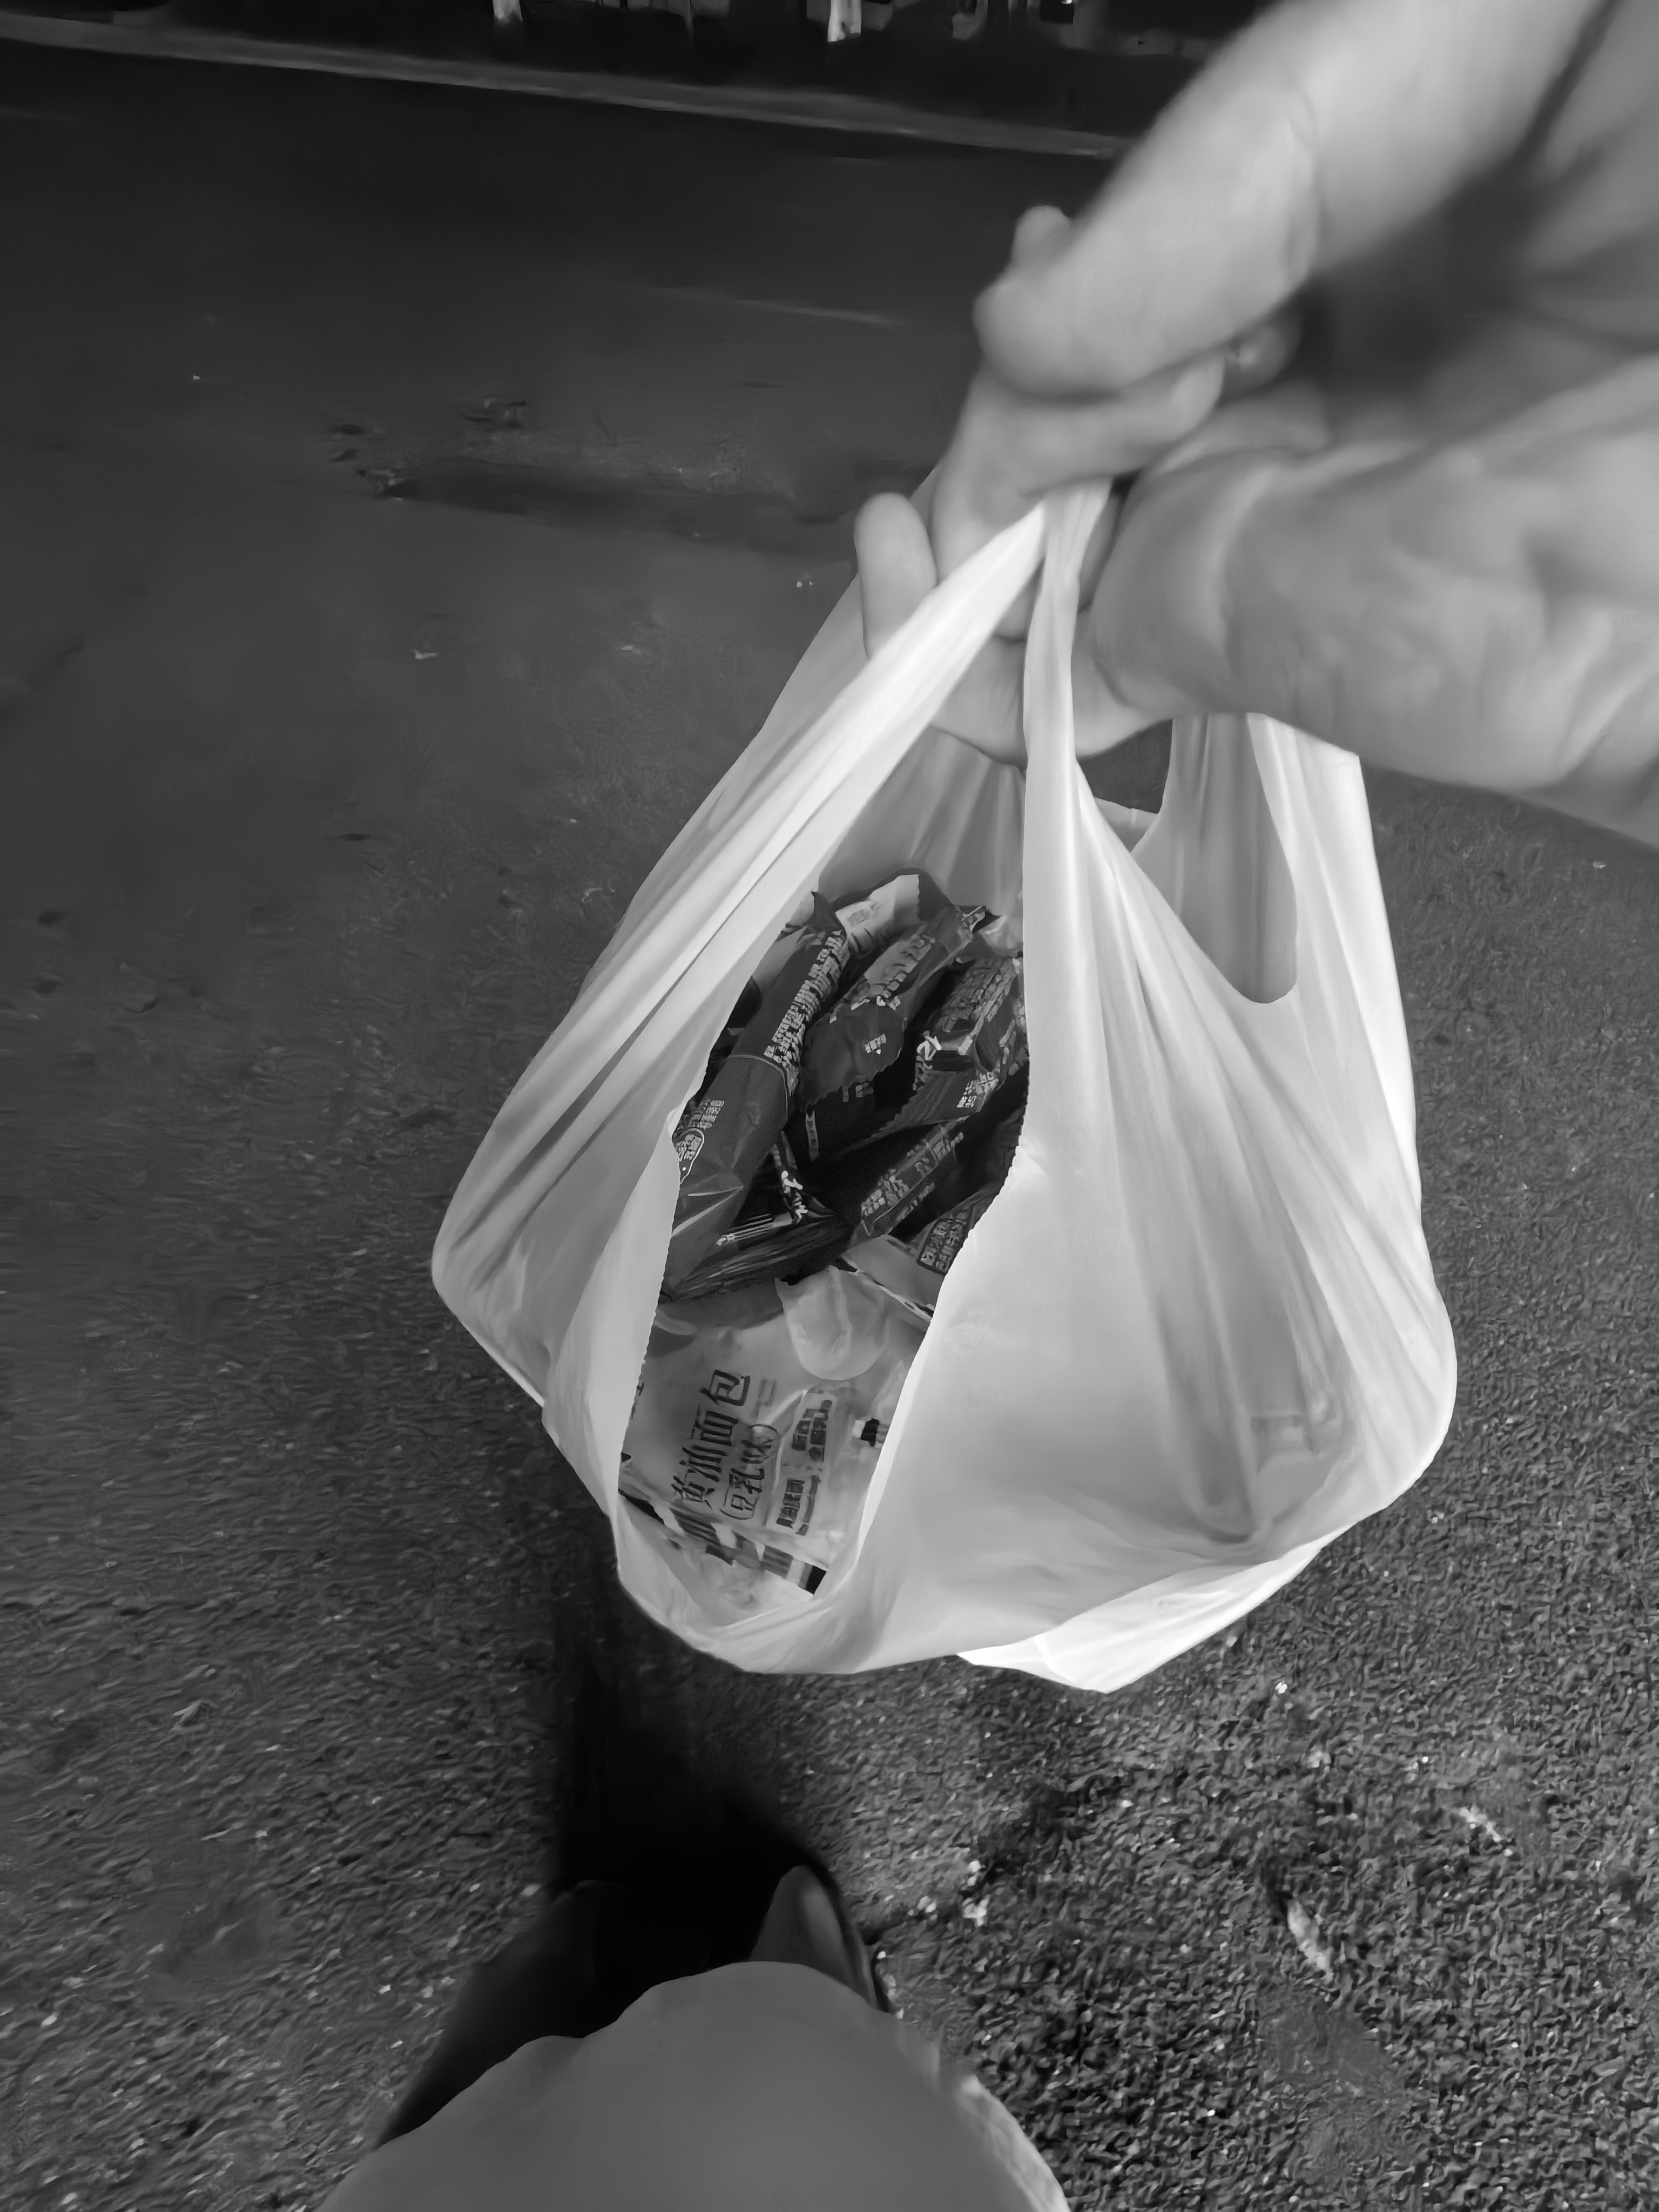
\includegraphics[width=\linewidth]{20250717.jpg} 
\end{wrapfigure}
\noindent
感觉长大了,\\
对零食的欲望也减少了,\\
在零食店转悠了半天,\\
好久不知道该买什么,\\
似乎没有小时候买零食的那股新鲜劲了,\\
最终倒也东拼西凑了一整袋。\\
不过有句话说的很好,\\
人总是在某一瞬间,发现自己不再是小孩。


\Date{2025}{7}{21}[\laughing]%
今天是好久不见的朋友聚会日,我感觉这个恐怖类型的密室逃脱,真的是越晚越害怕,今天玩人皮娃娃,全程担惊受怕,就是知道可能会有哪些吓人的,所有更加害怕,总是感觉哪里会吓你一下,哎,只能安慰自己是共情能力太强了,太容易沉浸式了。不过鸡哥还是很勇敢的,虽然我知道他也很害怕哈哈哈,也算是我们这群人之中的勇士了,今天还是很开心的,见到了久违的同学,再次相聚,感觉一切都没有变。
\begin{center}
    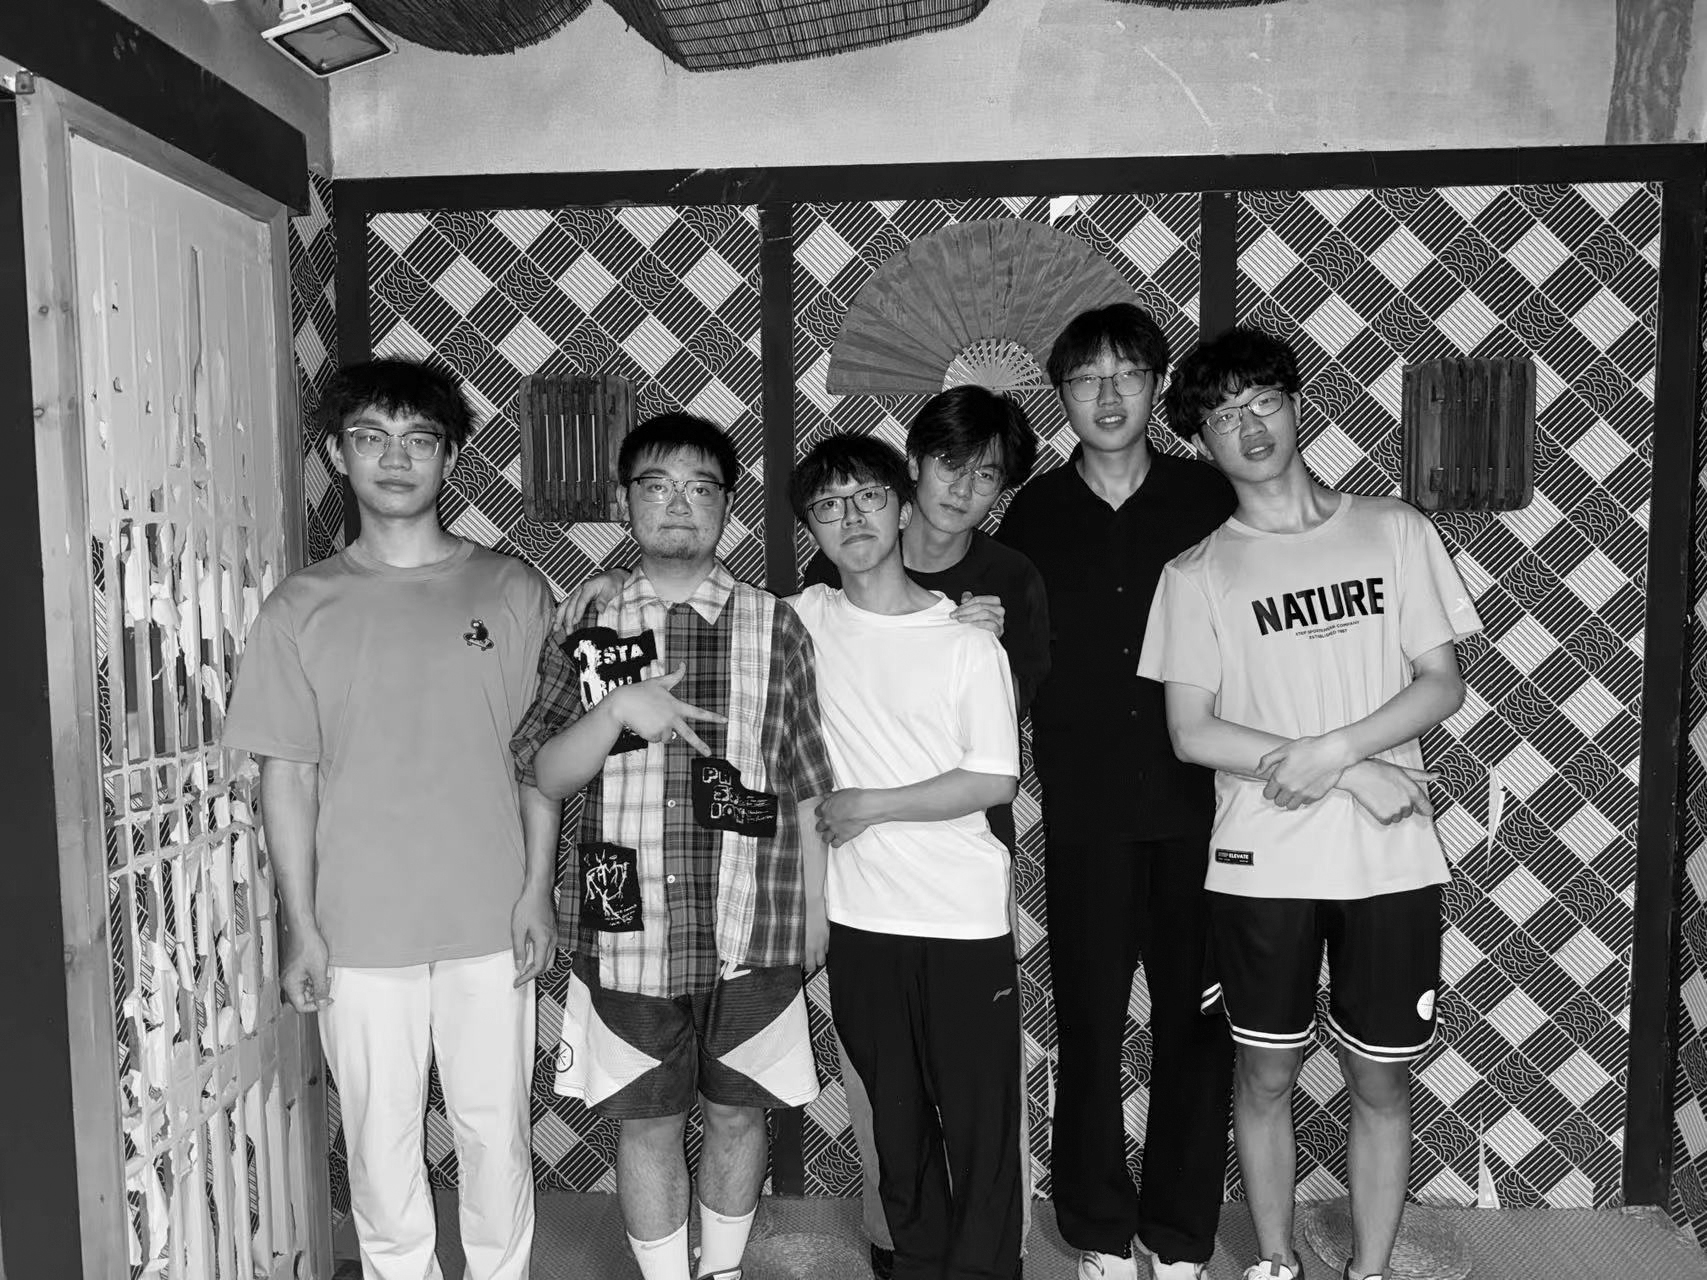
\includegraphics[width=0.8\linewidth,height=0.3\paperheight]{20250721.jpg}
\end{center}

\Date{2025}{8}{5}[\dizzy]%
今天的科目二考试真的很惊险刺激啊,第一次考的时候,刚进行第一个项目倒车入库,右倒库就车身出现不合格了,然后虽然有点小慌,还是直接开回起点没有走完第一次的全程,进行第二把,也是非常的惊险,我其实自己感觉车身还是有点多出线的,不过还是它没报错哈哈哈,赶忙驶出倒车入库的场地,一刻也不想多呆,后面的项目就很顺利了,一下子就嗖嗖嗖过了,总的来说还是过了的还是很不错的哈哈哈。

\Address[江苏][南京]
\Date{2025}{9}{9}[\confused]%
开学两周了,总是感觉不得劲,似乎总是会纠结一些无关紧要的事情,而在一些对自己很重要的事情上颓废。我想让自己慢下来,可似乎我又变成了拖延,我似乎也并不是很开心,但我也不知道要怎么才能开心起来,感觉一直都很迷茫,我不知道该做什么,但似乎我又知道,只是不愿意面对和行动。



\end{document}
%=================================天气指令==========================================%
% \sun 晴天太阳                  \sunny 晴朗                       \hot 炎热
% \windy 大风		  			   \clouds 多云  					   \snow 雪 
% \snowy 持续降雪  				 \snowyRainy 雨夹雪                \rainy 雨天 
% \rainySunny 太阳雨             \rainyThunder 雷阵雨 			 \thunderLight 闪电(无雨)  
% \hail 冰雹		               \dust 沙尘或雾霾
%
%=================================心情指令==========================================%
% \confused 困惑			       \sad 悲伤(难过或沮丧)             \simpleSmile 简单微笑
% \slightlySmile 淡淡微笑        \angry 生气                        \crying 哭泣(大哭或极度悲伤)
% \dizzy 晕眩                    \rage 暴怒                         \winkSmile 眨眼笑
% \stuckOutTongue 吐舌(调皮搞怪) \rollingEyes 翻白眼(无语或不耐烦) \confounded 苦恼
% \expressionless 无表情         \heartEyes 爱心眼(喜爱或迷恋)      \laughing 开怀大笑
% \nerdSmile 书呆子笑(呆萌或学霸) \openMouth 张嘴(惊讶或震惊)      \smirk 得意(狡猾或自满)
% \worried 担忧(忧虑或紧张)      \astonished 震惊(极度惊讶或目瞪口呆)

